\documentclass[border=3pt]{standalone}
\usepackage[T1]{fontenc}
\AtBeginDocument{\hyphenpenalty=10000 \exhyphenpenalty=10000 \pretolerance=-1 \tolerance=9999}
\usepackage{helvet}
\renewcommand{\familydefault}{\sfdefault}
\usepackage{amsmath,amssymb}
\usepackage[eulergreek]{sansmath}
\sansmath
\usepackage{tikz}
\usetikzlibrary{positioning,arrows.meta,calc,shapes.geometric,shapes.symbols,shapes.misc,backgrounds,patterns,decorations.pathreplacing,shadows.blur}
% ---------------- palette (distinct from the earlier manuscript)
\definecolor{ink}{HTML}{1D2B3A}
\definecolor{mute}{HTML}{6B7280}
\definecolor{line}{HTML}{CBD2D9}
\definecolor{sand}{HTML}{F7F3EC}
\definecolor{cor}{HTML}{E76F51}   % Stage 1 (endoscopy)
\definecolor{corl}{HTML}{FCE9E3}
\definecolor{sea}{HTML}{2A9D8F}   % Stage 2 (CT, PET, genomics)
\definecolor{seal}{HTML}{E0F2EF}
\definecolor{gold}{HTML}{D9A42B}  % data-integrity audits
\definecolor{goldl}{HTML}{FBF1D9}
\definecolor{nav}{HTML}{264653}   % reliability layer
\definecolor{navl}{HTML}{E3EAEE}
\definecolor{plum}{HTML}{8E5572}  % outputs to clinician
\definecolor{pluml}{HTML}{F3E8EE}
\tikzset{
  >={Stealth[length=2.4mm,width=1.8mm]},
  flow/.style={->, line width=0.9pt, draw=ink!70},
  thin/.style={->, line width=0.6pt, draw=mute},
  card/.style={draw=#1, line width=0.7pt, fill=white, rounded corners=3pt, blur shadow={shadow blur steps=5, shadow xshift=0.4mm, shadow yshift=-0.4mm, shadow opacity=18}},
  tag/.style={fill=#1, text=white, font=\tiny\bfseries, rounded corners=1.6pt, inner sep=1.6pt},
  hdr/.style={font=\scriptsize\bfseries, text=#1},
  sm/.style={font=\tiny, text=ink, align=center},
  smm/.style={font=\tiny, text=mute, align=center},
  num/.style={circle, fill=#1, text=white, font=\tiny\bfseries, inner sep=0.9pt, minimum size=4mm},
}

\graphicspath{{../assets/}}
\begin{document}
\begin{tikzpicture}[x=1mm,y=1mm]
\fill[sand, rounded corners=4pt] (-2,-31) rectangle (182,118);
% ---------------- headers
\foreach \x/\n/\t in {0/1/Patient inputs, 54/2/Modality tokens, 92/3/Masked self attention, 128/4/Fusion and task heads} {
  \node[num=sea] at (\x+2.5,113) {\n};
  \node[font=\scriptsize\bfseries, text=ink, anchor=west] at (\x+5.5,113) {\t};
}
\draw[line, line width=0.6pt] (0,109.5) -- (180,109.5);
% ---------------- (1) inputs with representative images
% CT
\node[font=\tiny\bfseries, text=ink, anchor=west] at (0,106.6) {Chest CT, axial slice};
\node[inner sep=0pt, anchor=south west] (ct) at (0,82) {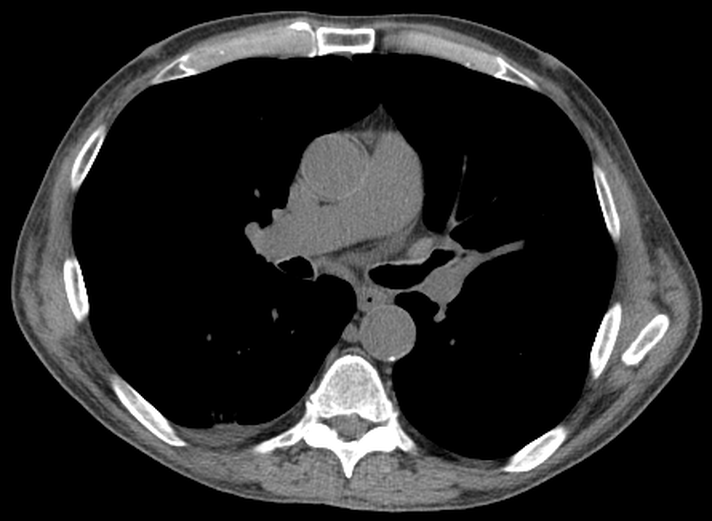
\includegraphics[width=30mm]{s2_ct.png}};
\draw[white, line width=0.6pt, -{Stealth[length=1.6mm]}] (24.5,101.4) -- (15.85,91.7);
\node[font=\fontsize{4.6}{5}\selectfont\bfseries, text=white, anchor=west] at (19.5,102.4) {esophagus};
% PET
\node[font=\tiny\bfseries, text=ink, anchor=west] at (0,79.6) {FDG PET/CT, fused};
\node[inner sep=0pt, anchor=south west] (pet) at (0,55) {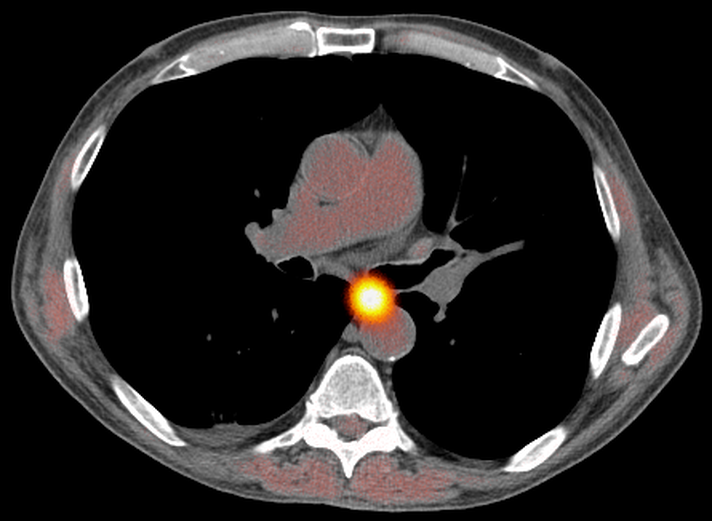
\includegraphics[width=30mm]{s2_pet.png}};
\draw[white, line width=0.6pt, -{Stealth[length=1.6mm]}] (24.5,74.6) -- (17.2,65.6);
\node[font=\fontsize{4.6}{5}\selectfont\bfseries, text=white, anchor=west] at (17.6,75.6) {focal uptake};
% Genomics
\node[font=\tiny\bfseries, text=ink, anchor=west] at (0,50.8) {Genomic profile};
\node[inner sep=0pt, anchor=south west] (gen) at (0,30) {
\includegraphics[width=30mm]{s2_geno.png}};
\node[font=\fontsize{4.4}{5}\selectfont, text=mute, anchor=north west] at (0,29.4) {1,500 features (30 $\times$ 50 grid)};
% availability badges
\foreach \y/\n/\p/\d in {93/34/17.1/512, 66/5/2.5/512, 39/180/90.5/{1,500}} {
  \node[font=\tiny\bfseries, text=ink, anchor=west] at (31.4,\y+3.6) {\n\,/\,199};
  \node[font=\fontsize{4.6}{5}\selectfont, text=mute, anchor=west] at (31.4,\y+0.6) {patients (\p\%)};
  \fill[line] (31.6,\y-2.6) rectangle (48.6,\y-1.4);
  \fill[sea] (31.6,\y-2.6) rectangle ({31.6+17*\p/100},\y-1.4);
  \node[font=\fontsize{4.6}{5}\selectfont, text=mute, anchor=west] at (31.4,\y-4.8) {\d{} dimensions};
}
% ---------------- (2) projection to tokens
\foreach \y/\lab/\sh/\st in {93/CT/35/solid, 66/PET/0/dashed, 39/G/45/solid} {
  \draw[flow] (49.4,\y) -- (54.4,\y);
  \node[draw=mute, fill=white, rounded corners=1.5pt, font=\tiny, text=ink, minimum width=14mm, minimum height=6.4mm, inner sep=1pt, align=center] at (62,\y) {Linear\\[0.5pt]LN, GELU};
  \draw[thin] (69.4,\y) -- (73.6,\y);
}
\node[circle, draw=sea, line width=0.8pt, fill=seal, minimum size=6mm, font=\tiny\bfseries, text=ink, inner sep=0pt] at (77.4,93) {CT};
\node[circle, draw=sea, line width=0.8pt, dashed, fill=white, minimum size=6mm, font=\tiny\bfseries, text=mute, inner sep=0pt] at (77.4,66) {PET};
\node[circle, draw=sea, line width=0.8pt, fill=sea!45, minimum size=6mm, font=\tiny\bfseries, text=ink, inner sep=0pt] at (77.4,39) {G};
\node[smm, text width=30mm] at (68,27.4) {one token of 256 dimensions per\\modality; a dashed token marks a\\modality absent for this patient};
% converge to attention
\draw[thin] (80.8,93) -- (85,93) -- (85,69);
\draw[thin] (80.8,39) -- (85,39) -- (85,63);
\draw[flow] (80.8,66) -- (92.4,66);
% ---------------- (3) masked attention grid
\begin{scope}[shift={(100,55)}]
  \foreach \r/\rl in {0/G,1/PET,2/CT} { \foreach \c/\cl in {0/CT,1/PET,2/G} {
     \pgfmathsetmacro{\w}{(\c==2)?72:38}
     \ifnum\c=1
       \fill[white] (\c*7.4,\r*7.4) rectangle ++(7,7);
       \fill[pattern=north east lines, pattern color=line] (\c*7.4,\r*7.4) rectangle ++(7,7);
     \else \fill[sea!\w] (\c*7.4,\r*7.4) rectangle ++(7,7); \fi } }
  \node[smm] at (3.5,24.2) {CT}; \node[smm] at (10.9,24.2) {PET}; \node[smm] at (18.3,24.2) {G};
  \node[smm, anchor=east] at (-0.6,18.3) {CT}; \node[smm, anchor=east] at (-0.6,10.9) {PET}; \node[smm, anchor=east] at (-0.6,3.5) {G};
  \node[smm] at (11,27.6) {keys};
\end{scope}
\node[smm, text width=36mm] at (111,45.6) {1 layer, 4 heads ($d_h$ = 64);\\key padding mask removes the\\absent modality (hatched)};
\draw[flow] (123.6,66) -- (128.6,66);
% ---------------- (4) fusion and heads
\node[draw=sea, fill=seal, line width=0.7pt, rounded corners=2pt, font=\tiny, text=ink, minimum width=20mm, minimum height=7mm, align=center] (mm) at (140,72) {masked mean\\[-1pt]$\sum_m\delta_m\tilde{\mathbf{e}}_m/\sum_m\delta_m$};
\node[draw=sea, fill=white, line width=0.7pt, rounded corners=2pt, font=\tiny, text=ink, minimum width=20mm, minimum height=7mm, align=center] (sh) at (140,57) {Linear(256$\rightarrow$128)\\[-1pt]LN, GELU};
\draw[thin] (mm) -- (sh);
\node[draw=sea, fill=sea, line width=0.8pt, rounded corners=2pt, font=\tiny\bfseries, text=white, minimum width=21mm, minimum height=7mm, align=center] (h1) at (168.5,72) {Subtype head\\[-1pt]{\fontsize{4.6}{5}\selectfont SCC vs.\ adenocarcinoma}};
\node[draw=mute, fill=white, line width=0.7pt, dashed, rounded corners=2pt, font=\tiny, text=mute, minimum width=21mm, minimum height=7mm, align=center] (h2) at (168.5,55) {Stage head\\[-1pt]{\fontsize{4.6}{5}\selectfont auxiliary, not an endpoint}};
\draw[thin] (sh.east) -- (153,57) |- (h1.west);
\draw[thin] (153,57) |- (h2.west);
\node[smm, text width=48mm] at (155,42.6) {heads trained with multisample dropout;\\CT and PET tokens dropped with $p$ = 0.15\\during training (one modality always kept)};
\node[font=\tiny\bfseries, text=sea!80!black] at (168.5,78.4) {nested CV AUROC 0.870};
% ---------------- illustration note
\node[font=\fontsize{4.6}{5}\selectfont, text=mute, anchor=west, text width=178mm, align=left] at (0,21.4) {Images are representative: CT from the public 3D Slicer chest sample; PET uptake simulated for illustration; genomic values illustrative. The model receives precomputed embeddings.};
% ---------------- bottom: missingness audit gate
\fill[goldl, rounded corners=3pt] (0,-29) rectangle (106,16);
\node[num=gold] at (3,12.2) {5};
\node[font=\scriptsize\bfseries, text=ink, anchor=west] at (6,12.2) {Missingness audit (before any endpoint is reported)};
\node[draw=gold, fill=white, line width=0.7pt, rounded corners=2pt, font=\tiny, text=ink, minimum width=21mm, minimum height=9mm, align=center] (q) at (14,-7) {does modality\\availability alone\\predict the label?};
\node[draw=sea, fill=seal, line width=0.8pt, rounded corners=2pt, font=\tiny, text=ink, text width=34mm, align=left, inner sep=2pt] (pass) at (51,2) {\textbf{Subtype}: availability only AUROC 0.561 vs.\ model 0.870; genomics only 0.867};
\node[draw=gold!90!black, fill=white, line width=0.8pt, rounded corners=2pt, font=\tiny, text=ink, text width=34mm, align=left, inner sep=2pt] (fail) at (51,-16) {\textbf{Staging}: stage readable for 32/199; recorded late cases cluster in patients with CT and no genomics};
\draw[thin] (q.east) -- (29,-7) |- (pass.west);
\draw[thin] (29,-7) |- (fail.west);
\node[tag=sea] at (95,2) {passes: reported};
\node[tag=gold!90!black] at (95,-16) {fails: excluded};
\draw[thin] (pass.east) -- (86.2,2);
\draw[thin] (fail.east) -- (86.6,-16);
% ---------------- bottom: nested cross-validation
\fill[seal, rounded corners=3pt] (110,-29) rectangle (180,16);
\node[num=sea] at (113,12.2) {6};
\node[font=\scriptsize\bfseries, text=ink, anchor=west] at (116,12.2) {Repeated nested cross validation};
\foreach \r in {0,1,2} {
  \node[font=\tiny, text=mute, anchor=east] at (122.6,3.2-\r*6.4) {rep \the\numexpr\r+1\relax};
  \foreach \f in {0,...,4} {
    \pgfmathtruncatemacro{\te}{mod(\r*2,5)}
    \ifnum\f=\te \fill[sea] (123.5+\f*10.4,1.6-\r*6.4) rectangle ++(9.8,3.4);
    \else \fill[white] (123.5+\f*10.4,1.6-\r*6.4) rectangle ++(9.8,3.4); \draw[sea!50, line width=0.4pt] (123.5+\f*10.4,1.6-\r*6.4) rectangle ++(9.8,3.4);
      \fill[gold!70] (123.5+\f*10.4+8.2,1.6-\r*6.4) rectangle ++(1.6,3.4); \fi
  }
}
\node[font=\tiny, text=ink, anchor=west] at (123,-18.6) {\tikz\fill[sea] (0,0) rectangle (2.6mm,1.8mm); outer test fold \quad \tikz\fill[gold!70] (0,0) rectangle (1.2mm,1.8mm); inner 15\% checkpoint split};
\node[smm, text width=66mm] at (145,-24.6) {3 repeats $\times$ 5 folds, 3 seeds per fold;\\every patient is scored by models that never saw that patient};
\end{tikzpicture}
\end{document}
